\documentclass[aps,pre]{revtex4-2}
\usepackage{amsmath}
\usepackage{bm}
\usepackage[ISO]{diffcoeff}
\usepackage{url}
\usepackage{amssymb}
\usepackage{hyperref}
\usepackage{graphicx}
\DeclareMathOperator{\diag}{diag}
\begin{document}
\title{Finite Element Method}
\author{Julian Fritzsch}
\affiliation{Department of Quantum Matter Physics, University of Geneva, CH-1211 Geneva, Switzerland}
\affiliation{School of Engineering, University of Applied Sciences of Western Switzerland, CH-1950 Sion, Switzerland}
\maketitle
\section{General Idea}\label{sec:general}
This chapter is basically a summary of~\cite{ferriteIntro, finiteelementspaces_2018}.
For a motivation of the finite element method we use the heat equation
\begin{align}
	-\nabla^2f(\bm{x})         & = \rho(\bm{x}), \qquad x\in\Omega,  \\
    f(\bm{x})                   & = f_D(\bm{x}), \qquad x\in\partial\Omega_D, \\
    \nabla f(\bm{x})\cdot\bm{n} & = f_N(\bm{x}), \qquad x\in\partial\Omega_N,
\end{align}
where $\partial\Omega_D$ is the part of the boundary where Dirichlet conditions are applied and $\partial\Omega_N$ is the part where Neumann conditions are applied ($\bm{n}$ is the outward facing normal).
This equation can be turned into the so-called weak form by multiplying with an arbitrary test function $g(\bm(x))$ and integrate over $\Omega$
\begin{align}
    -\int g(\bm{x}) \nabla (\nabla f(\bm{x})) \dl \Omega = -\int_{\partial\Omega} g(\bm{x})\nabla f(\bm{x})\bm{n}\dl \bm{x} + \int\nabla g(\bm{x})(\nabla f(\bm{x}))\dl\bm{x} = \int g(\bm{x})\rho(\bm{x}) \dl\Omega.
\end{align}
We demand that the test functions vanish on the boundary with Dirichlet conditions applied: $g(\bm{x}) = 0,\; \bm{x}\in\partial\Omega_D$.
It follows that
\begin{equation}\label{eq:weakform}
    \int\nabla g(\bm{x})(\nabla f(\bm{x}))\dl\bm{x} = \int_{\partial\Omega_N} g(\bm{x})f_N(\bm{x})\dl \bm{x} + \int g(\bm{x})\rho(\bm{x}).
\end{equation}
To discretize the functions we rewrite them as
\begin{equation}
	f(\bm{x}) \approx \sum_{i\in \mathcal{N}} f_i u_i(\bm{x}),\qquad g(\bm{x}) \approx \sum_{i\in \mathcal{N}} g_i u_i(\bm{x})\dl\Omega,\label{eq:expansion}
\end{equation}
where $\mathcal{N}$ denotes the set of all nodes, $f_i$ and $g_i$ are the nodal values and $u_i(\bm{x})$ are the shape functions that form a basis of the vector space.
We demand that the test functions fulfill $u_i(\bm{x}_j)=\delta_{ij}$, where $\bm{x}_i$ is the position of the $i$th node.
Inserting~\eqref{eq:expansion} into~\eqref{eq:weakform} yields
\begin{equation}
	\sum_{i,j}g_if_j\int\nabla u_i(\bm{x})(\nabla u_j(\bm{x})) \dl \Omega = \sum_{i}g_i\int_{\partial\Omega_N} u_i(\bm{x})f_N(\bm{x})\dl\bm{x} + \sum_{i}g_i\int u_i(\bm{x}) \rho(\bm{x})\dl\Omega.
\end{equation}
The above equation can be written in linearized form
\begin{equation}
    \bm{g}^\top\bm{K}\bm{f} = \bm{g}^\top\bm{\rho}.
\end{equation}
As this equation must hold for arbitrary $\bm{g}$ the problem can be solved by solving the linear equation
\begin{equation}
	\bm{K}\bm{f} = \bm{\rho}.
\end{equation}
The stiffness matrix $\bm{K}$ is given by
\begin{equation}
	\bm{K}_{ij} = \int\nabla u_i(\bm{x})(\nabla u_j(\bm{x})) \dl \Omega,
\end{equation}
the force vector $\bm{\rho}$ is given by
\begin{equation}
	\bm{\rho} = \int_{\partial\Omega_N} u_i(\bm{x})f_N(\bm{x})\dl\bm{x} + \int u_i(\bm{x}) \rho(\bm{x})\dl\Omega.
\end{equation}
To calculate the integrals we separate the space into elements (in our case triangles) and evaluate the integrals on each element.
This means the integration is turned into a sum of integrals over the different elements $\int\dl\Omega \to \sum_E\int\dl\Omega_E$.
The calculations can be simplified by defining the test functions on a reference element and then transforming them to fit the elements on our grid.
Typical vector spaces to approximate the solution space are the vector spaces of polynomials.
For our investigations we use linear polynomials.
Instead of using the basis $u_i = {1, x, y}$ we choose Lagrange polynomials that are defined by their nodal values.
For the unit triangle with nodes $P_1=(0,0)$, $P_2=(0,1)$, and $P_3=(1,0)$ they are given by
\begin{equation}
    \hat{u}_1(\hat{\bm{x}}) = \hat{x}, \quad \hat{u}_2(\hat{\bm{x}}) = \hat{y}, \quad \hat{u}_3(\hat{\bm{x}}) = 1 - \hat{x} - \hat{y}.
\end{equation}
The hat denotes that the quantity corresponds to a reference quantity.
It is straight forward to show that these functions satisfy our requirements.
The shape of the shape functions is shown in Fig.~\ref{fig:basefunctions}.
To transform the values of the shape functions of arbitrary cells onto the reference cell we map the reference position vector to the position vectors of the cell as
\begin{equation}
    \bm{x} = \bm{a} + \bm{B} \hat{\bm{x}} = h(\hat{\bm{x}}),
\end{equation}
where $\bm{a}$ and $\bm{B}$ are an appropriate vector and matrix, respectively.
An important property is that
\begin{equation}
    u_i(\bm{x}) = u_i(h(\hat{\bm{x}})) = \hat{u}_i(\hat{\bm{x}}).
\end{equation}
The gradient and the integration measure become
\begin{equation}
    \nabla u_i(\bm{x}) = \frac{1}{\det(J\hat{\bm{x}})}\nabla\hat{u}_i(\hat{\bm{x}}), \quad \dl\Omega_E = \det(J(\hat{\bm{x}}))\dl\hat{\bm{x}},
\end{equation}
where $J(\bm{x})$ is the Jacobian of $h(\bm{x})$.
For a more detailed description see~\cite{finiteelementspaces_2018}.

Finally we use a quadrature rule to evaluate the integrals.
This means the integral is approximated by weighted sum of the function evaluated at the quadrature points.
In our case we are using three quadrature points as shown in Fig.~\ref{fig:basefunctions} with weights $1/6$.
The integrals will then turn into sums over cells and quadrature points.
\begin{equation}
    \sum_E\int k\nabla u_i \nabla u_j \dl \Omega_E = \sum_E\sum_q\nabla \hat{u}_i(\hat{\bm{x}}_q) \nabla \hat{u}_j(\hat{\bm{x}}_q)\omega_q\frac{1}{\det(J(\hat{\bm{x}}_q))},
\end{equation}
where $\hat{\bm{x}}_q$ are the quadrature points, $\omega(\hat{\bm{x}}_q)$ are the quadrature weights.
The advantage is that we now only need to keep track of the transform between the cells and the references cell and do not need to evaluate the shape functions for each cell.
\begin{figure}
	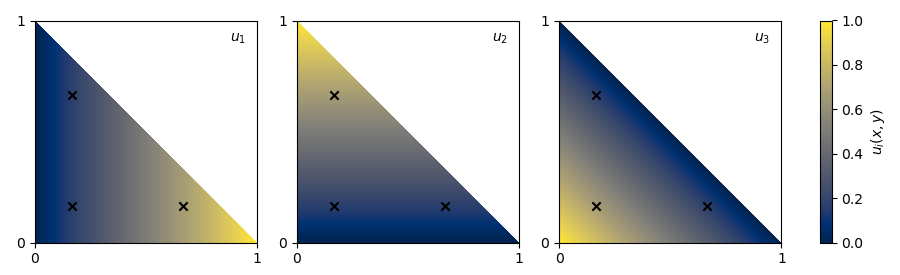
\includegraphics[width=.9\textwidth]{basisfunctions.png}
    \caption{Shape of the three shape functions for the unit triangle. The crosses show the location of the quadrature points.\label{fig:basefunctions}}
\end{figure}

\section{Application to the Swing Equations}
We want to apply the finite element method to our continuum model~\cite{pagnier_fritzsch_jacquod_chertkov_2022}
\begin{equation}\label{eq:swing}
	m(\bm{x})\ddot{\theta}(\bm{x}) + d(\bm{x})\dot{\theta}(\bm{x}) = p(\bm{x}) + \nabla\left(\begin{bmatrix}b_x(\bm{x}) & 0\\ 0 & b_y(\bm{x})\end{bmatrix}\nabla \theta(\bm{x})\right),
\end{equation}
where we have assumed that the susceptance tensor is diagonal.
The boundary conditions are given by
\begin{equation}
	\bm{n} \left(\begin{bmatrix}b_x(\bm{x}) & 0\\ 0 & b_y(\bm{x})\end{bmatrix}\nabla \theta(\bm{x})\right)= 0.
\end{equation}
Eq.~\eqref{eq:swing} can be rewritten as two first order differential equations (we are dropping the dependencies on $\bm{x}$ for the ease of reading)
\begin{equation}
	\begin{bmatrix}\mathbb{I} & 0\\0 & m\end{bmatrix}\partial_t\begin{bmatrix}\theta\\\omega\end{bmatrix} = \begin{bmatrix}\omega\\-d\omega + \nabla(\bm{B}\nabla \theta) + p\end{bmatrix},
\end{equation}
where $\bm{B} = \mathrm{diag}(b_x, t_y)$.

Using a similar approach as in the previous section, this equation reads in its weak form
\begin{equation}\label{eq:linearized}
	\begin{bmatrix}\bm{M}_1 & 0\\ 0 & \bm{M}_{2}\end{bmatrix}\partial_t\begin{bmatrix}\hat{\bm{\theta}} \\ \hat{\bm{\omega}}\end{bmatrix} = \begin{bmatrix}0 & \bm{K}_{12}\\\bm{K}_{21}&\bm{K}_{22}\end{bmatrix}\begin{bmatrix}\hat{\bm{\theta}}\\\hat{\bm{\omega}}\end{bmatrix} + \begin{bmatrix}0\\\bm{P}\end{bmatrix},
\end{equation}
where $\hat{\bm{\theta}}$ and $\hat{\bm{\omega}}$ are the vectors of the nodal values of $\theta$ and $\omega$.
The mass matrix is given by
\begin{equation}
	\bm{M}_{1, ij} = \int u_i(\bm{x})u_j(\bm{x})\dl\Omega, \qquad \bm{M}_{2, ij} = \int m(\bm{x})u_i(\bm{x})u_j(\bm{x})\dl\Omega.
\end{equation}
The stiffness matrices are given by
\begin{equation}
	\bm{K}_{12, ij} = \int u_i(\bm{x})u_j(\bm{x})\dl\Omega,\qquad \bm{K}_{21, ij} = -\int\nabla u_i(\bm{x})(\bm{B}(\bm{x})\nabla u_j(\bm{x}))\dl\Omega,
	\bm{K}_{22, ij} = -\int d(\bm{x}) u_i(\bm{x})u_j(\bm{x})\dl\Omega.
\end{equation}
Finally, the force vector is given by
\begin{equation}
	\bm{P}_i = \int p(\bm{x})u_i(\bm{x})\dl\Omega.
\end{equation}
It is important to notice that all matrices are time-independent such we only need to assemble these matrices once and can then use standard tools to solve~\eqref{eq:linearized}.

\section{Stable Solution and Machine Learning}
To obtain the stable solution for our problem we need to solve
\begin{equation}
	P(\bm{x}) + \nabla(\bm{B}\nabla\theta(\bm{x})) = 0.
\end{equation}
The weak form reads
\begin{equation}
	\bm{K}_{21} \hat{\bm{\theta}} = -\bm{P}.
\end{equation}
To ensure the well-posedness of the problem we need to enforce the value of $\hat{\bm{\theta}}$ on one node.
We set $\hat{\theta}_i = 0$, where $i$ is closest to the slack bus of the continuous system.
This corresponds to setting
\begin{equation}
	\bm{K}_{21, ij} = \bm{K}_{21, ji} = \delta_{ij}, \qquad \bm{P}_i = 0.
\end{equation}

We want to learn the parameters of $\bm{B}$ from the stable solutions of the system.
For this we need to rewrite $\bm{K}_{12}$ in vectorized form.
It turns out that we can write for a single cell
\begin{equation}\label{eq:decomposition}
    \bm{K}_\mathrm{cell} = \bm{A}_\mathrm{cell}\bm{B}^\prime_\mathrm{cell}\bm{A}^\top_\mathrm{cell},
\end{equation}
where (for three quadrature points per cell $\bm{x}_i$)
\begin{equation}
	\begin{split}
        \bm{A}_\mathrm{cell} =&
		\begin{bmatrix}
			\partial_x u_1(\bm{x}_1) & 0                        & \partial_x u_1(\bm{x}_2) & 0                        & \partial_x u_1(\bm{x}_3) & 0                        \\
			0                        & \partial_y u_1(\bm{x}_1) & 0                        & \partial_y u_1(\bm{x}_2) & 0                        & \partial_y u_1(\bm{x}_3) \\
			\partial_x u_2(\bm{x}_1) & 0                        & \partial_x u_2(\bm{x}_2) & 0                        & \partial_x u_2(\bm{x}_3) & 0                        \\
			0                        & \partial_y u_2(\bm{x}_1) & 0                        & \partial_y u_2(\bm{x}_2) & 0                        & \partial_y u_2(\bm{x}_3) \\
			\partial_x u_3(\bm{x}_1) & 0                        & \partial_x u_3(\bm{x}_2) & 0                        & \partial_x u_3(\bm{x}_3) & 0                        \\
			0                        & \partial_y u_3(\bm{x}_1) & 0                        & \partial_y u_3(\bm{x}_2) & 0                        & \partial_y u_3(\bm{x}_3)
		\end{bmatrix}\\
		&\cdot\diag\left(\sqrt{\det(\omega_1J(\bm{x}_1))},\sqrt{\det(\omega_1J(\bm{x}_1))},\sqrt{\det(\omega_2J(\bm{x}_2))},\right.\\
		&\left.\hphantom{\cdot\diag\big(}\sqrt{\det(\omega_2J(\bm{x}_2))},\sqrt{\det(\omega_3J(\bm{x}_3))},\sqrt{\det(\omega_3J(\bm{x}_3))} \right).
	\end{split}
\end{equation}
Note that this expression can be expanded to higher order quadrature rules.
It is important to point out that~\eqref{eq:expansion} needs the values of $\bm{b}$ in the quadrature points.
We deal with this the following way:
We provide the nodal values of $\bm{b}$ and project them onto the quadrature points.
This can be done in a straight forward fashion using the results of Section~\ref{sec:general}.
Using an appropriate projection matrix matrix $\bm{P}$ we can write
\begin{equation}
    \bm{B}^\prime_\mathrm{cell} = \bm{P}\diag\left(\bm{b}_x(\bm{x}_{N1}),\bm{b}_y(\bm{x}_{N1}),\bm{b}_x(\bm{x}_{N2}),\bm{b}_y(\bm{x}_{N2}),\bm{b}_x(\bm{x}_{N3}),\bm{b}_y(\bm{x}_{N3})\right),
\end{equation}
where $\bm{x}_{Ni}$ denotes the coordinates of the $i$th node.
Now we need to assemble the global matrix $\bm{A}$.
Each row corresponds to one node in the grid and we simply need to identify the local nodes of the elements with their global index.
The columns correspond to all the quadrature points that we can label arbitrarily, we just need to pay attention to correctly assemble the projection matrix.
By identifying the global index of the nodes of each cell and adding the values of $\bm{A}_\mathrm{cell}$ to the corresponding entries, $\bm{A}$ is constructed. 
To enforce the slack bus using this approach, we have to set the rows corresponding to the slack node to zero.
Finally, we add a matrix $\bm{C}$ that has a single entry on the diagonal at the slack bus node.
The stiffness matrix can then be written as
\begin{equation}
    \bm{K}_{21} = \bm{A}\bm{P}\bm{B}^\prime\bm{A}^\top + \bm{C}.
\end{equation}


\bibliography{bib}
\end{document}
